\documentclass[12pt, twoside]{article}
\usepackage[francais]{babel}
\usepackage[T1]{fontenc}
\usepackage[latin1]{inputenc}
\usepackage[left=7mm, right=7mm, top=7mm, bottom=7mm]{geometry}
\usepackage{float}
\usepackage{graphicx}
\usepackage{array}
\usepackage{multirow}
\usepackage{amsmath,amssymb,mathrsfs}
\usepackage{textcomp}
\pagestyle{empty}
\usepackage{soul}

\begin{document} 


\begin{center}
{\fbox{$4^{e}3$ \qquad \qquad \textbf{\Large{Devoir surveill� 6  (sujet 1) }}
\qquad \qquad 22/04/2011}}
\end{center}

\bigskip


\ul{\textbf{Exercice 1}}: (\textit{4 points})

\begin{enumerate}
  \item OUI est un triangle rectangle en O tel que OI=7dm et OU=24dm. Calculer
  la longueur manquante.
  \item DES est un triangle rectangle en D tel que DE=11,9mm et ES=16,9mm. Calculer
  la longueur manquante.  
\end{enumerate}

\bigskip





\ul{\textbf{Exercice 2}}: (\textit{4 points})


\enskip

Les angles $\widehat{OBD}$ et $\widehat{ORD}$ du quadrilat�re BORD sont-ils
droits? Justifier votre r�ponse.
 

\begin{center}
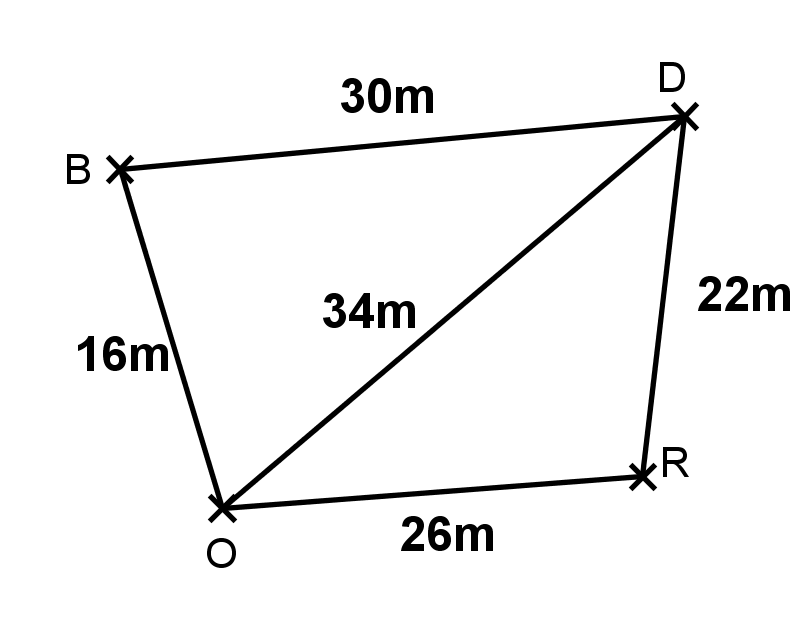
\includegraphics[width=7cm]{images/quadrilatere.png}
\end{center}


\bigskip


\ul{\textbf{Exercice 3}}: (\textit{4 points})

\enskip

Un potager a la forme d'un triangle rectangle et le jardinier veut
l'entourer d'une clot�re. Au moment de l'acheter, il s'aper�oit qu'il a oubli�
de mesurer un des c�t�s de l'angle droit. Les deux mesures dont il dispose sont
en m�tres: 6,75 et 10,59.

\begin{enumerate}
  \item A-t-il besoin d'aller mesurer le c�t� manquant? Pourquoi?
  \item Quelle est la longueur de la cl�ture �  acheter? Justifier votre
  r�ponse.
\end{enumerate}


\bigskip


\ul{\textbf{Exercice 4}}: (\textit{2+6 points})


\begin{tabular}{cc}
\begin{minipage}{10cm}
Les points A, O, F et C sont align�s.

 
AC=15cm; AO=OF=3cm; OB=6 cm. 

Les droites
(AC) et (BO) sont perpendiculaires.
\end{minipage}
&
\begin{minipage}{8cm}
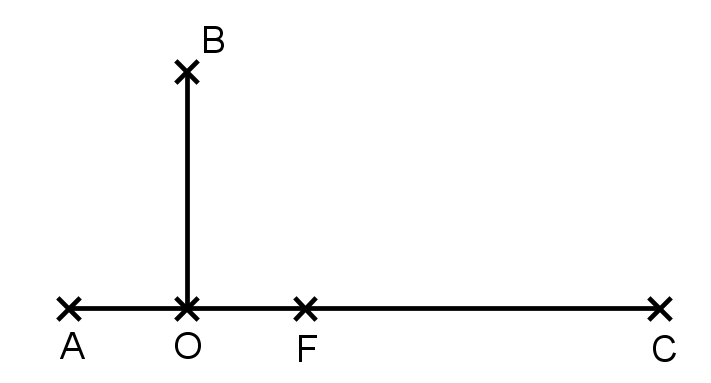
\includegraphics[width=6cm]{images/ex4.png}
\end{minipage}
\end{tabular}

 
\begin{enumerate}
  \item Construire la figure en vraie grandeur.
  \item Montrer que $AB^2=45$.
  \item Montrer que $BC^2=180$.
  \item Montrer que les droites (AB) et (BC) sont perpendiculaires.
  \item Tracer le cercle de diam�tre [FC], il coupe (BC) en H.
  \item Montrer que le triangle FHC est rectangle.
  \item Montrer que les droites (AB) et (FH) sont parall�les.
\end{enumerate}
 \pagebreak
 
 
 \begin{center}
{\fbox{$4^{e}3$ \qquad \qquad \textbf{\Large{Devoir surveill� 6  (sujet 2) }}
\qquad \qquad 22/04/2011}}
\end{center}

\bigskip


\ul{\textbf{Exercice 1}}: (\textit{4 points})

\begin{enumerate}
  \item MON est un triangle rectangle en O tel que MO=7cm et ON=5,25cm. Calculer
  la longueur manquante.
  \item SAM est un triangle rectangle en M tel que SA=58km et SM=42km.
  Calculer la longueur manquante.  
\end{enumerate}


\bigskip


\ul{\textbf{Exercice 2}}: (\textit{4 points})

 
\enskip

Les angles $\widehat{REC}$ et $\widehat{RIC}$ du quadrilat�re ERIC sont-ils
droits? Justifier votre r�ponse.
 

\begin{center}
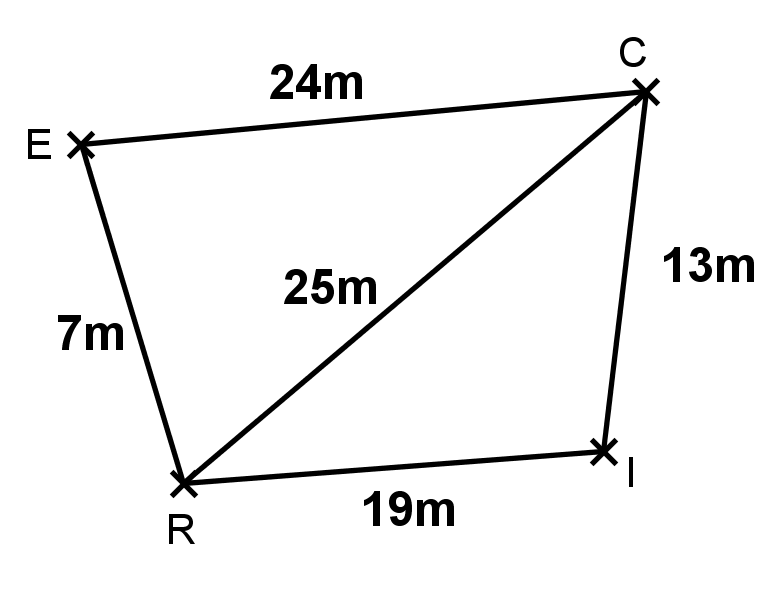
\includegraphics[width=6cm]{images/quadrilatere2.png}
\end{center}


\bigskip



\ul{\textbf{Exercice 3}}: (\textit{4 points})

\enskip

Un potager a la forme d'un triangle rectangle et le jardinier veut
l'entourer d'une clot�re. Au moment de l'acheter, il s'aper�oit qu'il a oubli�
de mesurer un des c�t�s de l'angle droit. Les deux mesures dont il dispose sont
en m�tres: 6,75 et 10,59.

\begin{enumerate}
  \item A-t-il besoin d'aller mesurer le c�t� manquant? Pourquoi?
  \item Quelle est la longueur de la cl�ture �  acheter? Justifier votre
  r�ponse.
\end{enumerate}



\bigskip


\ul{\textbf{Exercice 4}}: (\textit{2+6 points})


\begin{tabular}{cc}
\begin{minipage}{10cm}
Les points A, O, F et C sont align�s.

 
AC=15cm; AO=OF=3cm; OB=6 cm. 

Les droites
(AC) et (BO) sont perpendiculaires.
\end{minipage}
&
\begin{minipage}{8cm}
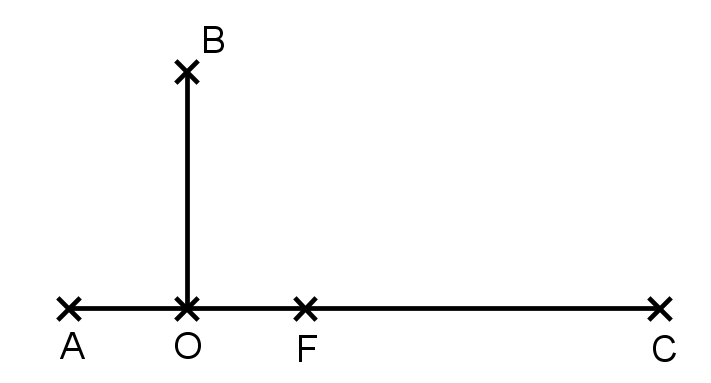
\includegraphics[width=6cm]{images/ex4.png}
\end{minipage}
\end{tabular}

 
\begin{enumerate}
  \item Construire la figure en vraie grandeur.
  \item Montrer que $AB^2=45$.
  \item Montrer que $BC^2=180$.
  \item Montrer que les droites (AB) et (BC) sont perpendiculaires.
  \item Tracer le cercle de diam�tre [FC], il coupe (BC) en H.
  \item Montrer que le triangle FHC est rectangle.
  \item Montrer que les droites (AB) et (FH) sont parall�les.
\end{enumerate}
\end{document}
